\subsection{Motion of a Point that moves relative to a Rigid Body}
\begin{frame}{Introduction}\vskip -8mm
	\begin{figure}[ht]
		\centering
		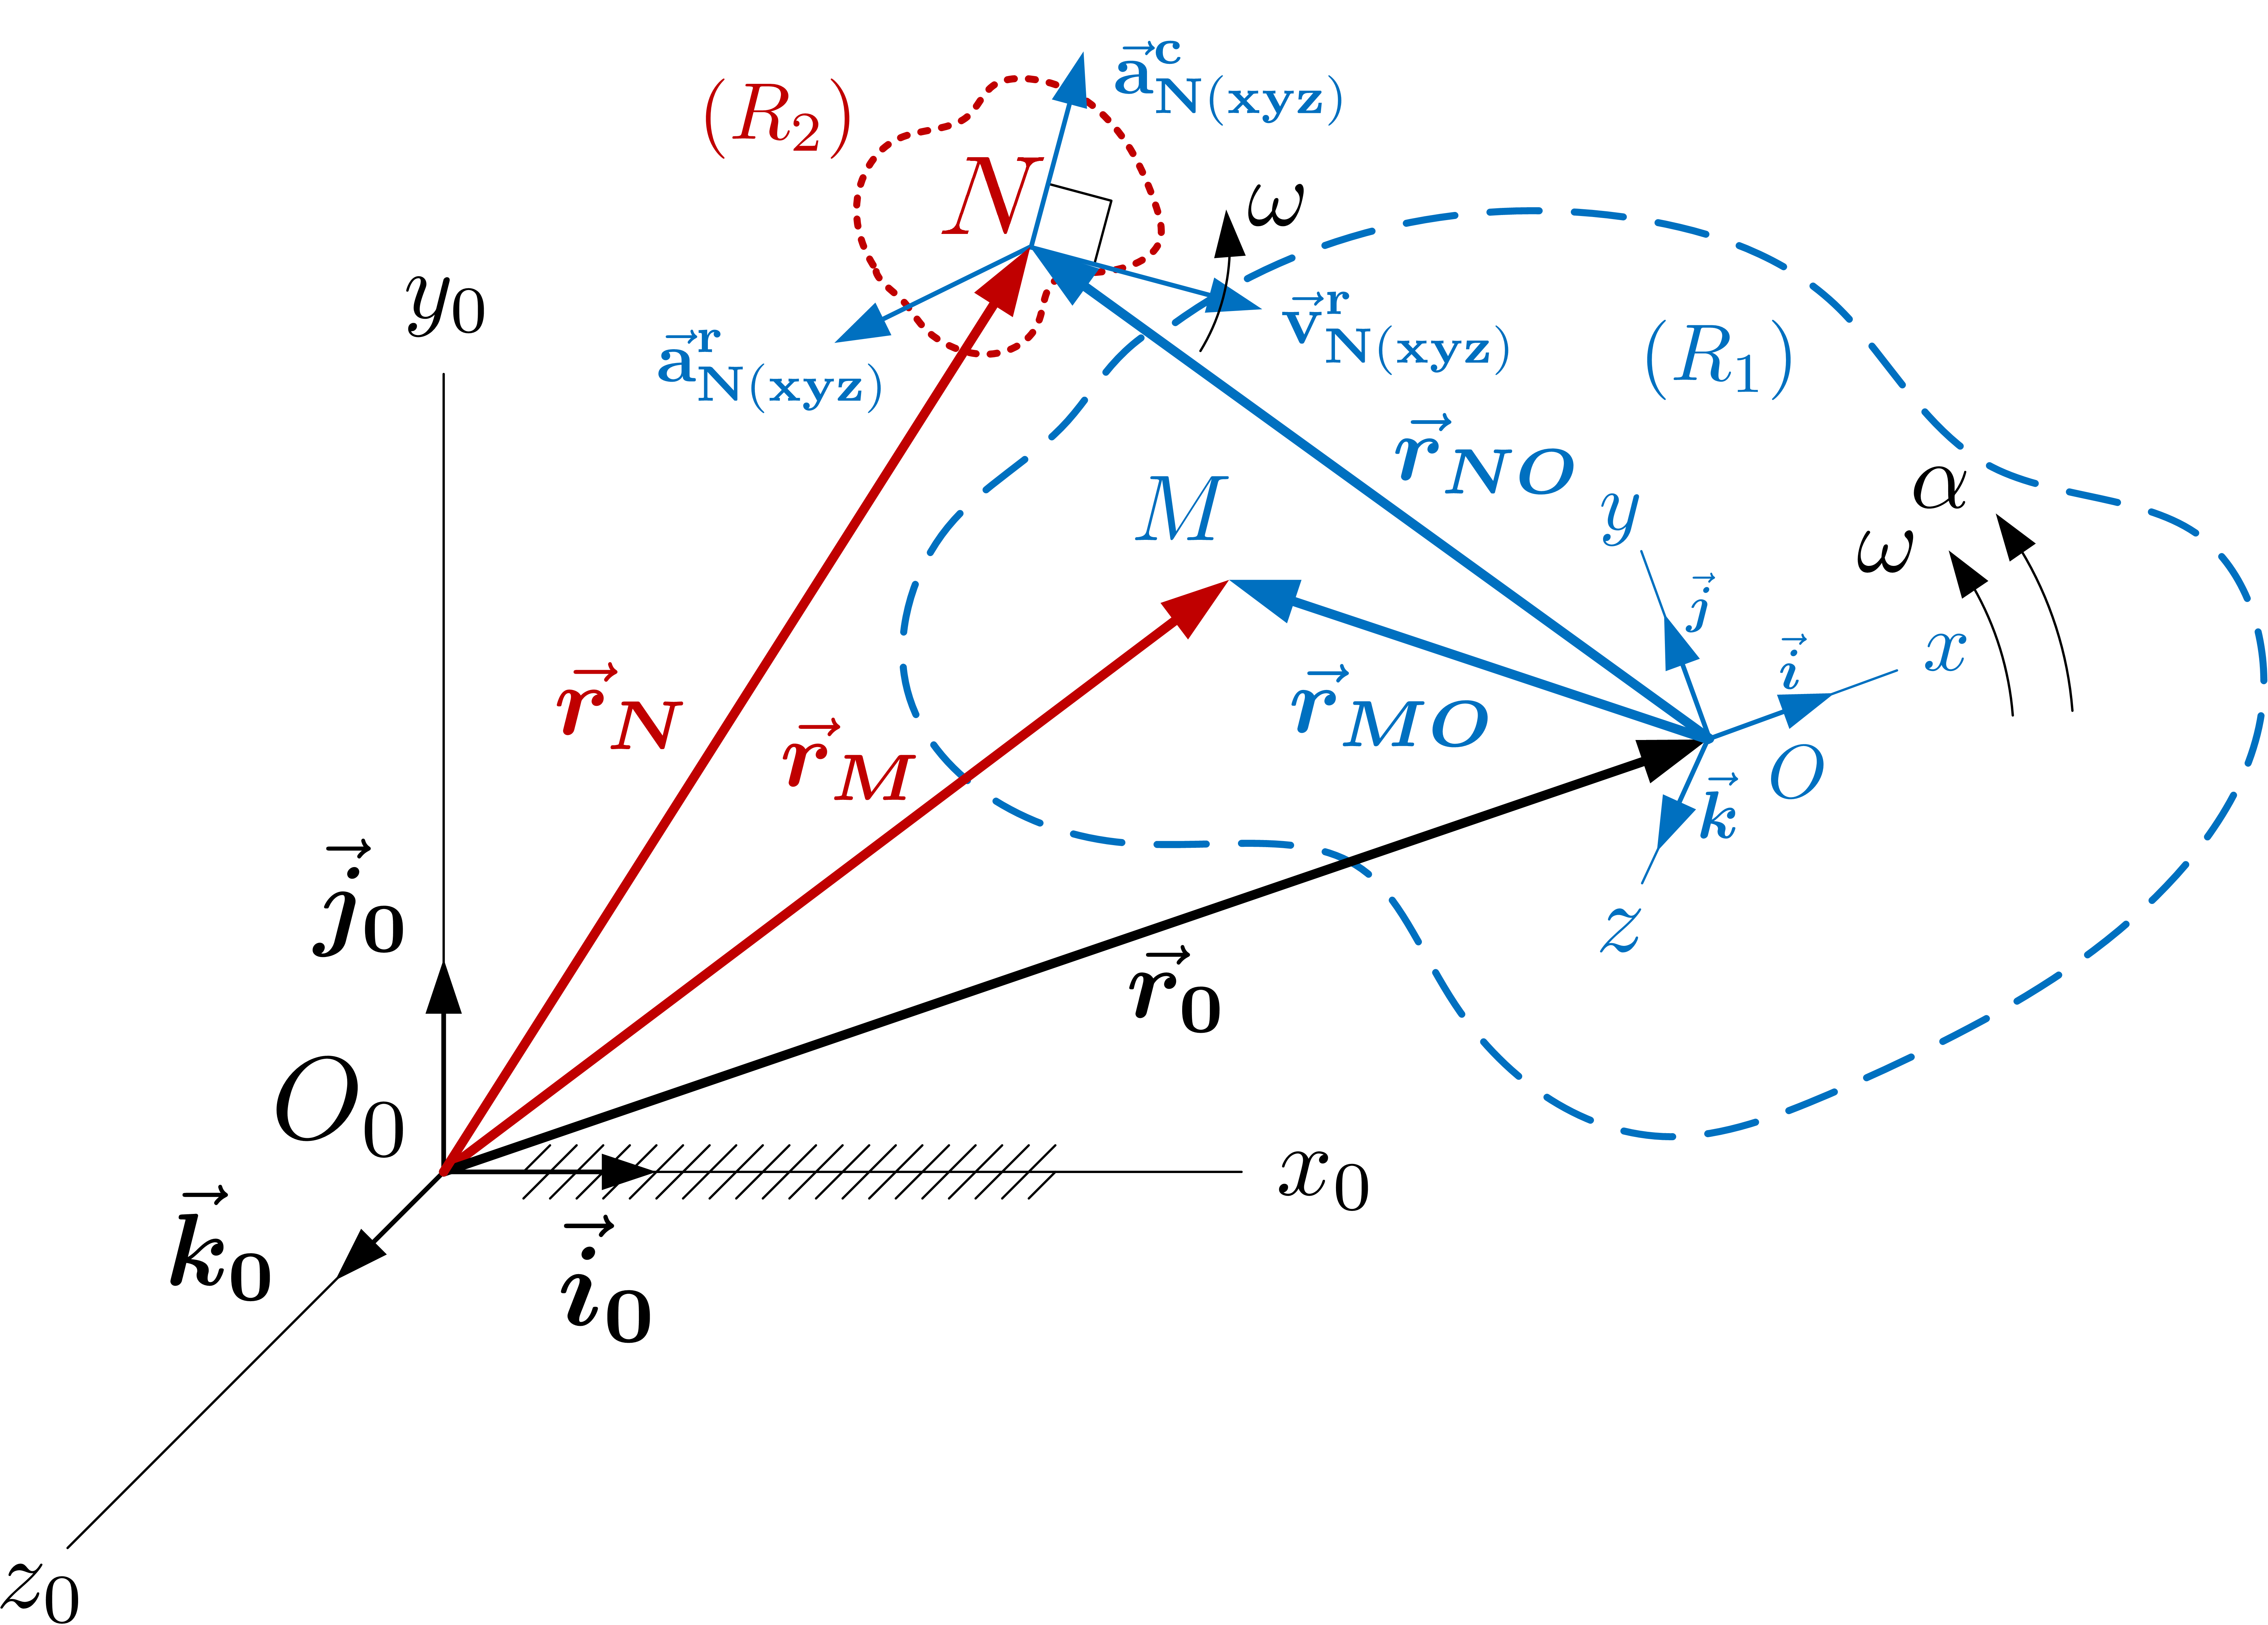
\includegraphics[width=80mm]{images/v_a_2.png}
	\end{figure}\vskip-4mm
	Position of point $N$ in rigid body $(R_2)$:
	\[\vb{r}{N}=\vb{r}{O}+\vb{r}{NO}=\vb{r}{O}+x\ih+y\jh+z\kh\]
\end{frame}
\begin{frame}
	Velocity vector $\vb{v}{N}$ of point $N$:\vskip1.25mm
	$\displaystyle\vb{v}{N}=\vb{v}{O}+[\dot{x}\ih+\dot{y}\jh+\dot{z}\kh]+[x\frac{d\ih}{dt}+y\frac{d\jh}{dt}+z\frac{d\kh}{dt}]$\\
	$\hskip 6.5mm\displaystyle=\vb{v}{O}+\vb{v}{N(xyz)}^{\bm r}+\vb{\omega}{}\times\vb{r}{}$\vskip2.5mm
	where $\vb{v}{N(xyz)}^{\bm r}$ is the relative velocity of point $N$ with respect to the reference frame of rigid body $(R_1)$.\vskip 5mm
	Acceleration vector $\vb{a}{N}$ of point $N$:\vskip1.25mm
	$\displaystyle\vb{a}{N}=\vb{a}{O}+[\ddot{x}\ih+\ddot{y}\jh+\ddot{z}\kh]+2\vb{\omega}{}\times\vb{v}{N(xyz)}^{\bm n}+\vb{\alpha}{}\times\vb{r}{}+\vb{\omega}{}\times(\vb{\omega}{}\times\vb{r}{})$\\
	$\hskip6.25mm\displaystyle= \vb{a}{O}+\vb{a}{N(xyz)}^{\bm r}+\vb{a}{N(xyz)}^{\bm c}+\vb{\alpha}{}\times\vb{r}{}+\vb{\omega}{}\times(\vb{\omega}{}\times\vb{r}{})$\\
	where:\\
	$\vb{a}{N(xyz)}^{\bm r}$ is the relative acceleration of point $N$ with respect to the reference frame of rigid body $(R_1)$.\\
	$\vb{a}{N(xyz)}^{\bm c}$ is referred to as \textit{Coriolis acceleration}.\vskip2.5mm
	For planar motions: $\displaystyle \vb{a}{O}= \vb{a}{O}+\vb{a}{N(xyz)}^{\bm r}+\vb{a}{N(xyz)}^{\bm c}+\vb{\alpha}{}\times\vb{r}{}-\vb{\omega}{}^2\vb{r}{}$
\end{frame}
\begin{frame}
	\begin{block}{Formulas}
		For any point $N$, its velocity and acceleration relative to a reference frame $O$ of a rigid body are:
		\[\begin{cases}
		\vb{v}{N}=\vb{v}{O}+\vb{v}{NO}^{\bm r}+\vb{\omega}{}\times\vb{r}{{NO}}\\
		\vb{a}{N}=\vb{a}{O}+\vb{a}{NO}^{\bm r}+2\vb{\omega}{}\times\vb{v}{NO}^{\bm r}+\vb{\alpha}{}\times\vb{r}{{NO}}+\vb{\omega}{}\times(\vb{\omega}{}\times\vb{r}{NO})
		\end{cases}\]
	\end{block}
\end{frame}